% Copyright 2004 by Till Tantau <tantau@users.sourceforge.net>.
%
% In principle, this file can be redistributed and/or modified under
% the terms of the GNU Public License, version 2.
%
% However, this file is supposed to be a template to be modified
% for your own needs. For this reason, if you use this file as a
% template and not specifically distribute it as part of a another
% package/program, I grant the extra permission to freely copy and
% modify this file as you see fit and even to delete this copyright
% notice. 

\documentclass{beamer}

% There are many different themes available for Beamer. A comprehensive
% list with examples is given here:
% http://deic.uab.es/~iblanes/beamer_gallery/index_by_theme.html
% You can uncomment the themes below if you would like to use a different
% one:

\usetheme{Madrid}
\usepackage{multirow}
\usepackage{graphicx} %package to manage images
\usepackage{caption}
\setbeamertemplate{caption}[numbered]
\usepackage{animate}
\usepackage{multicol}
\usepackage{makecell}
%\usepackage[utf8]{inputenc}
%\usepackage[english, vietnam]{babel}
\usepackage[utf8]{vietnam} 
\usepackage{enumitem}
\usepackage{tikz}
 
\newcommand*\mycirc[1]{%
   \begin{tikzpicture}
     \node[draw,circle,inner sep=1pt] {#1};
   \end{tikzpicture}}
\title[Đồ án tốt nghiệp]{Phương pháp học sâu giải bài toán phát hiện Malware}

% A subtitle is optional and this may be deleted

\author[Đặng Mạnh Cường]
{ \qquad  Sinh viên thực hiện \\ \qquad \vspace{0.5cm}Đặng Mạnh Cường   \\
\qquad Giáo viên hướng dẫn \\ 
\qquad  TS.Đinh Viết Sang}


\institute[HUST] % (optional, but mostly needed)
{
 % from CNTT2-04\\
  %Ha Noi University of Science and Technology
  }
% - Give the names in the same order as the appear in the paper.
% - Use the \inst{?} command only if the authors have different
%   affiliation.

\date{\qquad Hà Nội, 12-06-2018}

\AtBeginSubsection[]
{
  \begin{frame}<beamer>{Mục Lục}
    \tableofcontents[currentsection,currentsubsection]
  \end{frame}
}
\newenvironment<>{varblock}[2][\textwidth]{%
  \setlength{\textwidth}{#1}
  \begin{actionenv}#3%
    \def\insertblocktitle{#2}%
    \par%
    \usebeamertemplate{block begin}}
  {\par%
    \usebeamertemplate{block end}%
  \end{actionenv}}
% Let's get started
\begin{document}
\begin{frame}
  \titlepage
  
\end{frame}

\begin{frame}{Mục Lục}
  \tableofcontents
  % You might wish to add the option [pausesections]
\end{frame}

% Section and subsections will appear in the presentation overview
% and table of contents.
\section{Giới thiệu chung}
\begin{frame}{Malware là gì?}{Giới thiệu chung}
	Malware - malicious software là các phần mềm độc hại, có mục đích phá hoại máy tính người dùng
	\begin{figure}
		\centering
		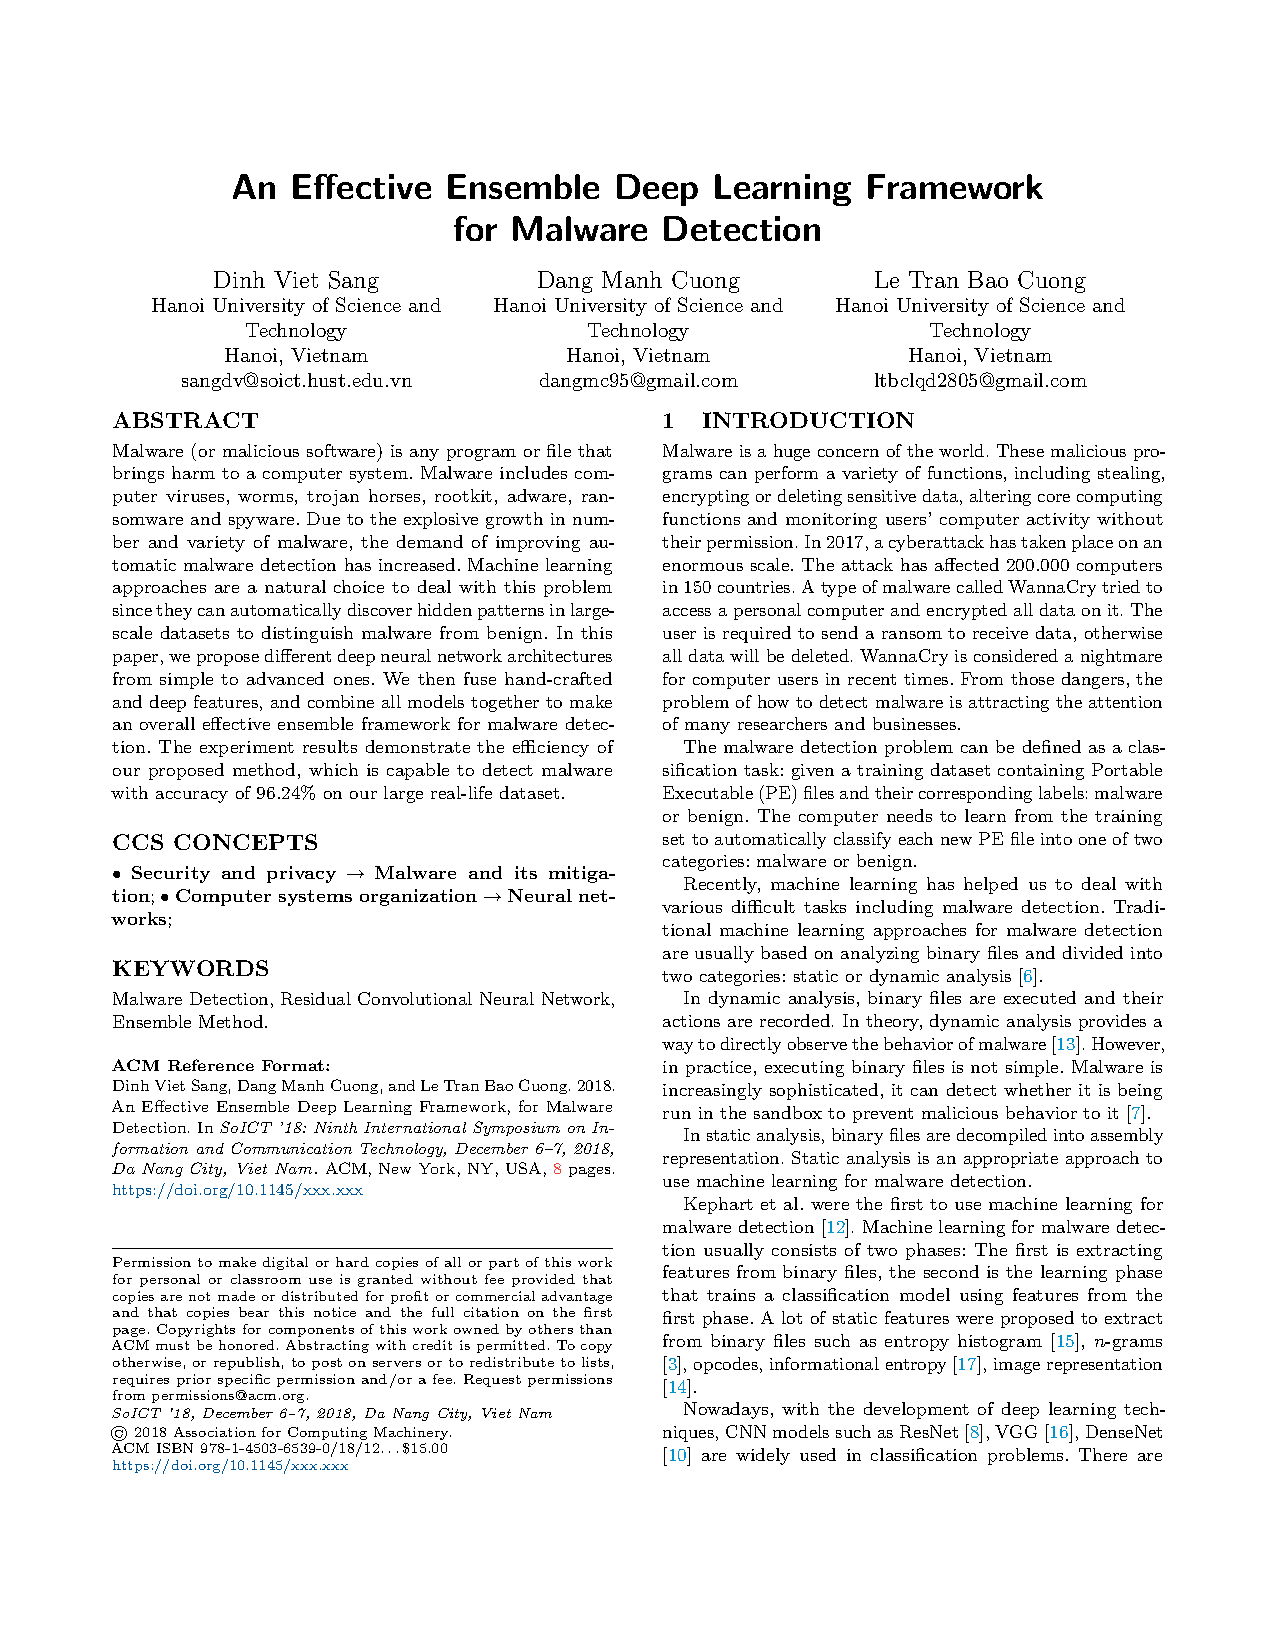
\includegraphics[width=0.7\textwidth]{malware.jpg}
		\caption{Các loại malware phổ biến}
		\label{fig:img1}
	\end{figure}
\end{frame}
\section{Bài toán phát hiện Malware}
\begin{frame}{Bài toán phát hiện Malware}
Cho tập dữ liệu đầu vào gồm các file PE, cần xác định mỗi mẫu PE có phải là malware hay không? \\
Về bản chất, bài toán phát hiện malware là bài toán phân loại nhị phân $\Rightarrow$ phân loại tập dữ liệu đầu vào thành 2 lớp:
\begin{itemize}[label=\textbullet]
	\item malware
	\item benign
\end{itemize}
\end{frame}


% Phương pháp tiếp cận
\section{Phương pháp tiếp cận}
\begin{frame}{Phương pháp tiếp cận}
Phương pháp này đưa chia làm 2 giai đoạn chính:
\begin{itemize}[label=\textbullet]
	\item Trích chọn đặc trưng
	\item Huấn luyện
\end{itemize}
\end{frame}
% Trích chọn đặc trưng
\subsection{Trích chọn đặc trưng}
\begin{frame}{Trích chọn đặc trưng}{Phương pháp tiếp cận}
	\begin{figure}
		\centering
		\includegraphics[width=0.7\textwidth]{TSPDs/report/binary_file.png}
		\caption{Biểu diễn PE dưới dạng mã máy}
		\label{fig:pe}
	\end{figure}
\end{frame}
\begin{frame}{Trích chọn đặc trưng}{Phương pháp tiếp cận}
Các đặc trưng:
\begin{itemize}[label = \textbullet]
	\item N-gram
	\item Entropy histogram
	\item Biểu diễn ảnh
	\item Lời gọi hệ thống (trích chọn trực tiếp từ file PE)
\end{itemize}
\end{frame}
\begin{frame}{N-gram}{Trích chọn đặc trưng}
\begin{itemize}[label = \textbullet]
	\item N-gram được sử dụng để biểu diễn tần suất xuất hiện của n bytes liên tiếp trong chuỗi bytes ban đầu.
	\item Không gian lưu trữ, độ phức tạp tính toán tỉ lệ thuận với n \\ $\Rightarrow$ chọn n = 1
	\item Vector đặc trưng kích thước 256 biểu diễn tần suất xuất hiện của từng bytes.
\end{itemize}
\end{frame}
\begin{frame}{Entropy histogram}{Trích chọn đặc trưng}
\begin{itemize}[label=\textbullet]
\item Entropy histogram được đề xuất bởi Joshua Saxe, đặc trưng này biểu
diễn sự xuất hiện của cặp byte dữ liệu và giá trị entropy của chuỗi byte chứa nó.\\
\item Quá trình trích xuất như sau:
\begin{itemize}[label=\textendash]
	\item Chia chuỗi bytes ban đầu thành n đoạn, mỗi đoạn có kích thước 1024 bytes.
	\item Với mỗi đoạn, xây dựng vector $v$ kích thước 1024, mỗi phần tử $v_i$ là cặp giá trị ($x,y$), trong đó $x$ là giá trị byte dữ liệu tương ứng với vị trí $i$ trong đoạn, $y$ là giá trị entropy của đoạn. 
	\item Sử dụng histogram để xây dựng vector đặc trưng 256 chiều dựa trên các vector tương ứng với mỗi đoạn trên.
\end{itemize}
\end{itemize}
\end{frame}
\begin{frame}{Entropy histogram}{Trích chọn đặc trưng}
\begin{figure}
		\centering
		\includegraphics[width=0.7\textwidth]{TSPDs/report/histogram.png}
		\caption{Histogram}
		\label{fig:his}
	\end{figure}
Giá trị của mỗi ô ($x,y$) trên hình biểu diễn tần suất xuất hiện của cặp giá trị ($x,y$) $\Rightarrow$ vector đặc trưng 256 chiều.
\end{frame}
\begin{frame}{Biểu diễn ảnh}{Trích chọn đặc trưng}
\begin{itemize}[label=\textbullet]
	\item Phương pháp biểu diễn file nhị phân dưới dạng ảnh được đề xuất bởi J.Nataraj.
	\item Mỗi byte trong file nhị phân tương ứng với giá trị một pixel trong ảnh.
	\item Duyệt hết toàn bộ file, thu được ảnh xám.
	\item Kích thước ảnh phụ thuộc vào kích thước file.
\end{itemize}
\end{frame}
\begin{frame}{Biểu diễn ảnh}{Trích chọn đặc trưng}
\begin{table}[ht]
    \centering
    \caption{Kích thước ảnh tương ứng với kích thước file nhị phân}
    \label{tab:size}
    \begin{tabular}{|c|c|} % <-- Alignments: 1st column left, 2nd middle and 3rd right, with vertical lines in between
      \hline
      \textbf{Kích thước file (KB)} & \textbf{Chiều rộng ảnh} \\
      \hline
      < 10 & 32\\
      \hline
      10 - 30 & 64\\
      \hline
      30 - 60 & 128\\
      \hline
      60 - 100 & 256\\
      \hline
      100 - 200 & 384\\
      \hline
      200 - 500 & 512\\
      \hline
      500 - 1000 & 784\\
      \hline
      > 1000 & 1024\\
      \hline
    \end{tabular}
\end{table}
Để phù hợp với mô hình huấn luyện $\Rightarrow$ đưa các ảnh về cùng kích thước \\64 $\times$ 64
\end{frame}
\begin{frame}{Lời gọi hệ thống}{Trích chọn đặc trưng}
\begin{itemize}[label=\textbullet]
	\item Lời gọi hệ thống là các hàm hệ thống (api) được các file PE sử dụng để thực hiện một số hành vi nhất định.
	\item Sự xuất hiện của các hàm này có thể cung cấp thông tin cho việc phát hiện malware.
	\item Sử dụng tập 794 api được phân tích từ 500,000 mẫu malware $\Rightarrow$ xây dựng vector đặc trưng 794 chiều biểu diễn sự xuất hiện của các api trong mỗi mẫu PE.
\end{itemize}
\end{frame}
% Mô hình áp dụng
\subsection{Mô hình áp dụng}
\begin{frame}{Mô hình áp dụng}{Phương pháp tiếp cận}
Sử dụng 2 kiến trúc mạng nơ-ron nhân tạo:
\begin{itemize}[label=\textbullet]
	\item Deep Neural Nerworks (DNN): đối với 3 đặc trưng N-gram, ENT-HIS, api.
	\item Residual Neural Networks (RESNETS): đối với đặc trưng ảnh và sự kết hợp của cả 4 đặc trưng
\end{itemize}
\end{frame}
% Thực nghiệm
\begin{frame}{Deep Neural Networks}{Mô hình áp dụng}
\begin{figure}
		\centering
		\includegraphics[width=0.6\textwidth]{TSPDs/report/dnn.png}
		\caption{Mô hình DNN}
		\label{fig:his}
	\end{figure}
\end{frame}
\begin{frame}{Deep Neural Networks}{Mô hình áp dụng}
\begin{table}[ht]
\centering
\caption{Kiến trúc mô hình với mỗi đặc trưng}
\label{tab:struct}
\begin{tabular}{|c|c|c|c|}
\hline
Đặc trưng & \multicolumn{3}{c|}{Kiến trúc mô hình}                                                                       \\ \hline
          & \begin{tabular}[c]{@{}c@{}}Số lượng units \\       lớp ẩn\end{tabular} & Hàm kích hoạt & Batch normalization \\ \hline
N-gram    & 128                                                                    & Relu          & Có                  \\ \hline
ENT-HIS   & 128                                                                    & Relu          & Có                  \\ \hline
API       & 256                                                                    & Relu          & Có                  \\ \hline
\end{tabular}

\end{table}
\end{frame}
\begin{frame}{Residual Neural Networks}{Mô hình áp dụng}
\begin{itemize}[label=\textbullet]
	\item Resnets được giới thiệu lần đầu tiên vào năm 2015 bởi Kaiming He cùng nhóm nghiên cứu tại Microsoft.
	\item Ý tưởng chính của Resnets là sử dụng \textbf{shortcut connection}.
\end{itemize}
	\begin{figure}
		\centering
		\includegraphics[width=0.6\textwidth]{TSPDs/report/res_block.png}
		\caption{Residual block}
		\label{fig:his}
	\end{figure}
\end{frame}
\begin{frame}{Residual Neural Networks}{Mô hình áp dụng}
\begin{figure}
		\centering
		\includegraphics[width=0.2\textwidth]{TSPDs/report/residual2.png}
		\caption{Residual block}
		\label{fig:his}
	\end{figure}
\end{frame}
\begin{frame}{Residual Neural Networks}{Mô hình áp dụng}
\begin{figure}
		\centering
		\includegraphics[width=1\textwidth]{TSPDs/report/rnsimg.png}
		\caption{Kiến trúc mô hình RNSIMG}
		\label{fig:his}
	\end{figure}
\end{frame}
\begin{frame}{Residual Neural Networks}{Mô hình áp dụng}
	\begin{figure}
		\centering
		\includegraphics[width=0.6\textwidth]{TSPDs/report/esrnsall.png}
		\caption{Mô hình RNSALL}
		\label{fig:his}
	\end{figure}
\end{frame}
\section{Thực nghiệm và đánh giá}
\begin{frame}{Dữ liệu thực nghiệm}{Thực nghiệm và đánh giá}
Bộ dữ liệu bao gồm 28,000 mẫu PE. Trong đó, 14,000 mẫu malware được thu thập
trên trang Virusshare - cộng đồng chia sẻ malware miễn phí, 14,000 mẫu benign được
thu thập từ các máy tính nội bộ thuộc Tập Đoàn Công nghiệp \& Viễn Thông Quân Đội
Viettel. Bộ dữ liệu được chia thành 2 tập:
\begin{itemize}[label=\textbullet]
	\item Tập huấn luyện: gồm 10,500 mẫu malware và 10,500 mẫu benign
	\item Tập đánh giá: gồm 3,500 mẫu malware và 3,500 mẫu benign
\end{itemize}
\end{frame}

\begin{frame}{Môi trường thực nghiệm}{Thực nghiệm và đánh giá}
Các thử nghiệm đánh giá được thực hiện trên hệ điều hành Ubuntu 16.04 với các thông số như sau:
\begin{itemize}[label=\textbullet]
	\item Ram 8GB.
 	\item Ổ cứng HDD 1TB.
 	\item Card đồ họa GeForce GTX 1080.
\end{itemize}
\end{frame}

\begin{frame}{Nội dung thực nghiệm}{Thực nghiệm và đánh giá}
\begin{itemize}[label=\textbullet]
	\item So sánh hiệu năng của các mô hình DNN-Ngram, DNN-EH, DNN-API, RNSIMG, RNSALL, ENSEMBLE.
	\item Độ chính xác của các mô hình được đánh giá bằng k-Fold crossvalidation, k= 10.
	\item Các mô hình này được huấn luyện bằng Momemtum Gradient descent với các tham số được thiết lập như sau:
	\begin{itemize}[label=\textendash]	
		\item Số lần lặp: 40000
		\item Batch size: 64
		\item Weight decay: 0.005
		\item Learning rate khởi tạo 0.001, giảm đi 1 nửa sau mỗi 10000 lần lặp
	\end{itemize}
\end{itemize}
\end{frame}

\begin{frame}{Kết quả thực nghiệm}{Thực nghiệm và đánh giá}
\begin{figure}
		\centering
		\includegraphics[width=1\textwidth]{TSPDs/report/result.png}
		\caption{Hiệu năng của các mô hình}
		\label{fig:his}
	\end{figure} 
\end{frame}
\begin{frame}{Kết quả thực nghiệm}{Thực nghiệm và đánh giá}
\begin{table}[ht]
\centering
\caption{Bảng các giá trị \textbf{True/False Positive/Negative} của các mô hình}
\label{tab:TP}
\begin{tabular}{|c|c|c|c|c|}
\hline
\multirow{2}{*}{Mô hình} & \multicolumn{2}{c|}{Dự đoán malware} & \multicolumn{2}{c|}{Dự đoán benign} \\ \cline{2-5} 
                         & TP                & FP               & FN               & TN               \\ \hline
DNN-Ngram                & 3232              & 240              & 268              & 3260             \\ \hline
DNN-EH                   & 3300              & 160              & 200              & 3340             \\ \hline
DNN-API                  & 3363              & 314              & 137              & 3186             \\ \hline
RNSIMG                   & 3222              & 156              & 278              & 3344             \\ \hline
RNSALL                   & 3316              & 156              & 184              & 3344             \\ \hline
\textbf{ENSEMBLE}        & \textbf{3386}     & \textbf{149}     & \textbf{114}     & \textbf{3351}    \\ \hline
\end{tabular}

\end{table}       
\end{frame}
\section{Kết luận và hướng phát triển}
\begin{frame}{Kết luận và hướng phát triển}
\begin{itemize}[label=\textbullet]
	\item Cài đặt, thử nghiệm, đánh giá các mô hình DNN-Ngram, DNN-EH, DNN-API, RNSIMG, RNSALL.
	\item Kết quả cho thấy sự kết hợp của cả 4 đặc trựng cho kết quả tốt hơn các đặc trưng riêng lẻ, đạt 95,14\% trên tập đánh giá.
	\item Ngoài ra, việc kết hợp các mô hình với nhau cho kết quả tốt hơn, mô hình ENSEMBLE đạt 96,24\% trên tập đánh giá.
	\item Trong tương lại cần xây dựng bộ dữ liệu lớn hơn, cải thiện độ chính xác của các mô hình để có thể đưa vào sử dụng trong thực tế.
\end{itemize}
\end{frame}



\begin{frame}
\Huge 
\begin{center}
	THANK YOU!
\end{center}
\end{frame}
\end{document}

